\subsection{Helligkeitsverteilung}
\begin{table}[h!]
    \centering
    \begin{tabular}{ | l | c | c | c |}
        \hline
        Konfiguration & Beste & Unter 50 kB & Unter 28 kB \\\hline
        Ensemble-Methode & ExtraTrees & ExtraTrees & ExtraTrees \\\hline
        Maximalhöhe & 14 & 10 & 15 \\\hline
        Waldgröße & 10 & 6 & 1 \\\hline
        min\_samples\_leaf & 4 & 4 & 4 \\\hline
        Programmgröße in Bytes & 76628 & 33284 & 9364 \\\hline
        Genauigkeit Testmenge von Klisch & 74,0\% & 63,5\% & 67,7\% \\\hline
        Genauigkeit Gestentestmenge & 74,1\% & 79,2\% & 76,6\% \\\hline
        Genauigkeit Nullgestentestmenge & 69,0\% & 71,0\% & 67,0\% \\\hline
    \end{tabular}
    \caption{Beste Konfigurationen der Helligkeitsverteilung.}
    \label{tab:helligkeitsverteilung}
\end{table}
\begin{figure}[h!]
    \centering
    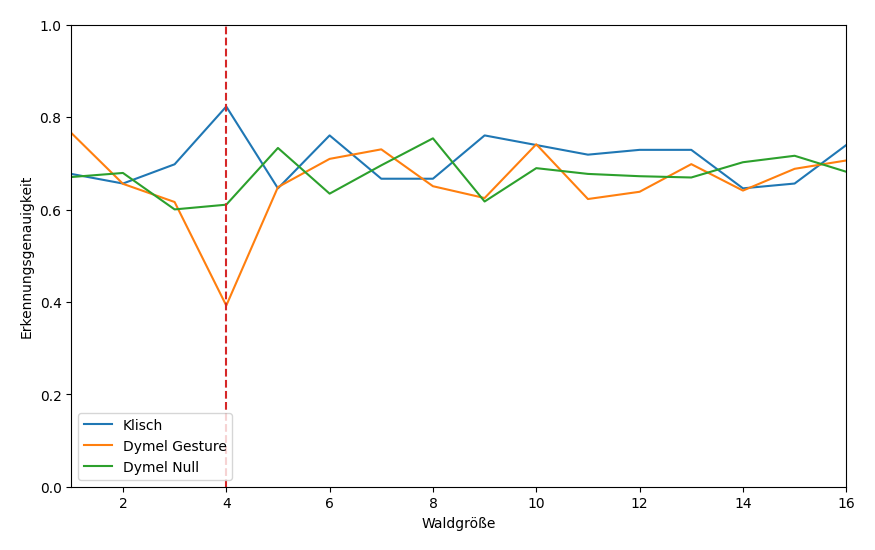
\includegraphics[width=\linewidth]{images/helligkeitsverteilung_acc_per_size.png}
    \caption{Die beste summierte Erkennungsgenauigkeit pro Waldgröße mit der Helligkeitsverteilung.}
    \label{fig:helligkeitsverteilung_per_forest_size}
\end{figure}
Die Featuremenge der Helligkeitsverteilung beinhaltet insgesamt 12 Features. Jeweils 6 Feature repräsentieren Zeitfenster der Minimalen Helligkeit und der Maximalen Helligkeit. Die Zeitfenster wurden
geometrisch zusammengefasst.
\newline
\newline
Die beste Konfiguration wurde mit der ExtraTrees Ensemble-Methode gefunden (siehe Tabelle \ref{tab:helligkeitsverteilung}). Sie erzielt eine Erkennungsgenauigkeit von $82,3\%$ auf der Testmenge von Klisch
und ist damit nur $17,7\%$ schlechter als das neuronale Netzwerk von Giese \cite{gieseThesis}. Außerdem klassifiziert diese Konfiguration $61\%$ aller Nullgesten aus der Testmenge von Dymel korrekt und ist
damit in Summe deutlich besser als die anderen Ensemble-Methoden. Allerdings ist die Erkennungsgenauigkeit auf der Gestentestmenge von Dymel nur bei $39,2\%$, wobei RandomForest deutlich besser ist mit
einer Erkennungsgenauigkeit von $55,4\%$. Insgesamt hat RandomForest damit ein besseres balanciertes Ergebnis, da die Erkennungsgenauigkeit auf dei Nulltestmenge und Testmenge von Klisch nur leicht
schlechter sind als die der Extra-Tress Methode. Mit einer Programmgröße von 4560 Bytes und 25844 Bytes passen beide Konfigurationen, ohne Optimierungen vorzunehmen, auf das Arduino Board.
\newline
\newline
Abbildung \ref{fig:helligkeitsverteilung_per_forest_size} zeigt keinen nennenswerten Anstieg der Erkennungsgenauigkeit durch eine größere Waldgröße.